\documentclass[tikz, preview]{standalone}
\usepackage{amsfonts, amsthm, amssymb, amsmath, stmaryrd, etoolbox}
\usepackage{tikz}
\usetikzlibrary{matrix,arrows}
\tikzset{->-/.style={decoration={markings, mark=at position .5 with {\arrow{>}}},postaction={decorate}}}
\tikzset{->-pos/.style={decoration={markings, mark=at position #1 with {\arrow{>}}},postaction={decorate}}}
\tikzset{->-/.style={decoration={markings,mark=at position .5 with {\arrow{>}}},postaction={decorate}}}
\tikzset{->-pos/.style={decoration={markings,mark=at position #1 with {\arrow{>}}},postaction={decorate}}}

\begin{document}
%%%%%%%%%%%%%%%%% 
%%%%%%%%%%%%%%%%% 
\[
  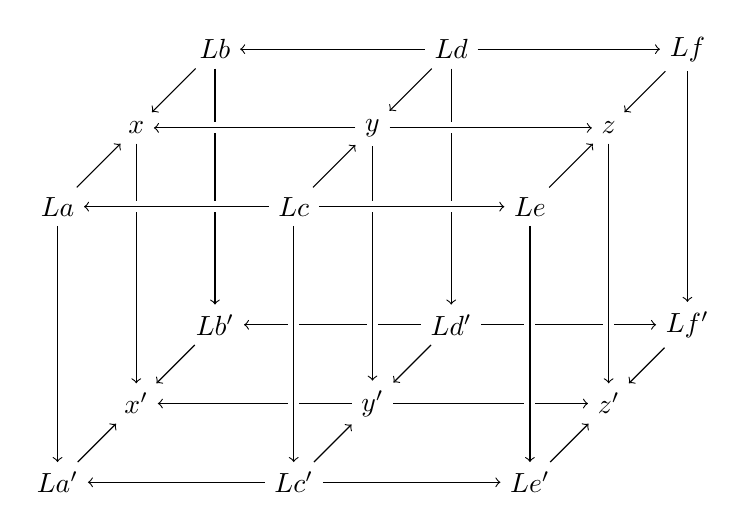
\begin{tikzpicture}
    % \draw [help lines, step=0.5, color=blue!10] (-5,-5) grid (5,5); % grid
    % 
    \node (t1) at (-2,2) {$ Lb $};
    \node (t2) at (-3,1) {$ x $};
    \node (t3) at (-4,0) {$ La $};
    \node (t4) at (1,2) {$ Ld $};
    \node (t5) at (0,1) {$ y $};
    \node (t6) at (-1,0) {$ Lc $};
    \node (t7) at (4,2) {$ Lf $};
    \node (t8) at (3,1) {$ z $};
    \node (t9) at (2,0) {$ Le $};
    \node (b1) at (-2,-1.5) {$ Lb' $};
    \node (b2) at (-3,-2.5) {$ x' $};
    \node (b3) at (-4,-3.5) {$ La' $};
    \node (b4) at (1,-1.5) {$ Ld' $};
    \node (b5) at (0,-2.5) {$ y' $};
    \node (b6) at (-1,-3.5) {$ Lc' $};
    \node (b7) at (4,-1.5) {$ Lf' $};
    \node (b8) at (3,-2.5) {$ z' $};
    \node (b9) at (2,-3.5) {$ Le' $};
    % 
    \draw [->] (t1) to node [] {$  $} (b1);
    \draw [->] (t4) to node [] {$  $} (b4);
    \draw [->] (t7) to node [] {$  $} (b7);
    \draw [->] (t4) to node [] {$  $} (t1);
    \draw [->] (t4) to node [] {$  $} (t7);
    \draw [->] (b4) to node [] {$  $} (b1);
    \draw [->] (b4) to node [] {$  $} (b7);
    \draw [->] (t1) to node [] {$  $} (t2);
    \draw [->] (t4) to node [] {$  $} (t5);
    \draw [->] (t7) to node [] {$  $} (t8);
    \draw [->] (b1) to node [] {$  $} (b2);
    \draw [->] (b4) to node [] {$  $} (b5);
    \draw [->] (b7) to node [] {$  $} (b8);
    \draw [->] (t2) to node [] {$  $} (b2);
    \draw [line width=4.0pt,color=white] (t5) -- node [] {$  $} (b5);
    \draw [->] (t5) to node [] {$  $} (b5);
    \draw [line width=4.0pt,color=white] (t8) -- node [] {$  $} (b8);
    \draw [->] (t8) to node [] {$  $} (b8);
    \draw [line width=4.0pt,color=white] (t5) -- node [] {$  $} (t2);
    \draw [->] (t5) to node [] {$  $} (t2);
    \draw [line width=4.0pt,color=white] (t5) to node [] {$  $} (t8);
    \draw [->] (t5) to node [] {$  $} (t8);
    \draw [->] (b5) to node [] {$  $} (b2);
    \draw [->] (b5) to node [] {$  $} (b8);
    \draw [->] (t3) to node [] {$  $} (t2);
    \draw [->] (t6) to node [] {$  $} (t5);
    \draw [->] (t9) to node [] {$  $} (t8);
    \draw [->] (b3) to node [] {$  $} (b2);
    \draw [->] (b6) to node [] {$  $} (b5);
    \draw [->] (b9) to node [] {$  $} (b8);
    \draw [line width=4.0pt,color=white] (t6) -- node [] {$  $} (t3);
    \draw [->] (t6) to node [] {$  $} (t3);
    \draw [line width=4.0pt,color=white] (t6) --  node [] {$  $} (t9);
    \draw [->] (t6) to node [] {$  $} (t9); 
    \draw [->] (b6) to node [] {$  $} (b3);
    \draw [->] (b6) to node [] {$  $} (b9);
    \draw [line width=4.0pt,color=white] (t3) -- node [] {$  $} (b3);
    \draw [->] (t3) to node [] {$  $} (b3);
    \draw [line width=4.0pt,color=white] (t6) -- node [] {$  $} (b6);
    \draw [->] (t6) to node [] {$  $} (b6);
    \draw [line width=4.0pt,color=white] (t9) -- node [] {$  $} (b9);
    \draw [->] (t9) to node [] {$  $} (b9);
  \end{tikzpicture}
\]
%%%%%%%%%%%%%%%%% 
%%%%%%%%%%%%%%%%% 
\end{document}
